\chapter{Analyse et Conception}
\label{chap:analyse}

\section{Introduction}

La phase d'analyse des besoins et de conception logicielle constitue l'étape déterminante permettant de traduire les exigences métier et les contraintes opérationnelles du domaine hôtelier dans un langage formel, standardisé et non ambigu. Dans le cadre de l'ingénierie d'une plateforme microservices distribuée comme le \textbf{PMS AMH Hospitality}, une modélisation rigoureuse est indispensable pour garantir la cohérence des flux transactionnels, la modularité des services et l'étanchéité des données entre établissements.

Ce chapitre expose l'ensemble de la démarche d'ingénierie système adoptée. Nous débuterons par la présentation du langage de modélisation standard UML, puis nous détaillerons l'étude critique de l'existant, la matrice RACI des acteurs du système, le diagramme global des cas d'utilisation et les fiches descriptives textuelles de chaque scénario critique. Nous présenterons ensuite les diagrammes de séquence dynamiques illustrant les flux d'authentification biométrique, de réservation concurrente et de clôture nocturne, pour achever sur le diagramme de classes du domaine métier et la cartographie des contextes délimités (\textit{Bounded Contexts}) issue des principes du \textit{Domain-Driven Design} (DDD).

\section{Présentation du langage de modélisation UML}

La Figure~\ref{fig:logo_uml} présente l'emblème du langage standard de modélisation logicielle.

\begin{figure}[H]
\centering
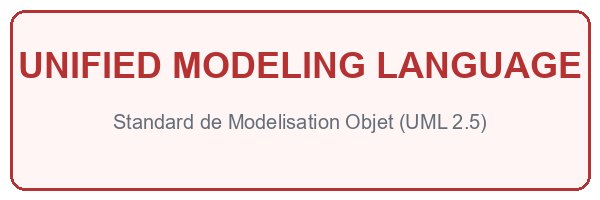
\includegraphics[width=0.5\textwidth]{figures/logo_uml.png}
\caption{Logo UML (\textit{Unified Modeling Language})}
\label{fig:logo_uml}
\end{figure}

Le langage UML (\textit{Unified Modeling Language}), standardisé internationalement par l'\textit{Object Management Group} (OMG, version 2.5), constitue le formalisme visuel universel de référence pour la spécification, la visualisation, la construction et la documentation des artefacts logiciels orientés objet. 

Dans le cadre de notre projet, UML a été mobilisé pour modéliser trois vues complémentaires du système :
\begin{itemize}
    \item \textbf{La vue fonctionnelle} : À travers les \textit{diagrammes de cas d'utilisation} et leurs fiches textuelles associées, permettant de cadrer les frontières du système et les interactions avec les utilisateurs hôteliers ;
    \item \textbf{La vue comportementale et dynamique} : À travers les \textit{diagrammes de séquence}, permettant de tracer chronologiquement l'ordonnancement des messages échangés entre les composants clients, la passerelle d'API, les microservices, le cache Redis et les bases de données relationnelles ;
    \item \textbf{La vue structurelle et statique} : À travers les \textit{diagrammes de classes}, permettant de formaliser les concepts du domaine métier hôtelier, leurs attributs typés, leurs opérations et les relations cardinales qui les lient.
\end{itemize}

\section{Étude et critique de l'existant opérationnel}

L'audit organisationnel et fonctionnel approfondi mené au sein des Riads du groupe AMH Hospitality à Marrakech a mis en évidence les limites majeures des processus manuels et des outils artisanaux précédemment utilisés. Le Tableau~\ref{tab:critique_existant_detail} synthétise l'analyse causale \textbf{Dysfonctionnement $\rightarrow$ Impact Opérationnel $\rightarrow$ Besoin Fonctionnel Ciblé}.

\begin{table}[H]
\centering
\small
\renewcommand{\arraystretch}{1.3}
\begin{tabularx}{\textwidth}{|p{3.8cm}|p{4.2cm}|X|}
\hline
\textbf{Dysfonctionnement Observé} & \textbf{Impacts et Risques Opérationnels} & \textbf{Besoin Fonctionnel Ciblé} \\
\hline
Synchronisation manuelle des plateformes OTA (Booking, Airbnb) & Surréservations (\textit{overbooking}), litiges clients à l'arrivée, dégradation de la réputation en ligne, pénalités financières. & Moteur de réservation centralisé avec verrouillage distribué Redis (anti-collision) et passerelle Channel Manager. \\
\hline
Clôture journalière (Night Audit) manuelle sur tableur & Erreurs de calcul sur la TVA et les taxes locales (TS/TPT), durée d'exécution excessive ($> 1$h30), risque d'asymétrie financière. & Moteur d'audit transactionnel automatisé avec calcul fiscal strict, rollback en cas d'anomalie et archivage S3 immuable. \\
\hline
Partage de comptes génériques sur les postes de réception & Impossibilité d'imputer les erreurs de saisie ou de caisse, traçabilité nulle, vulnérabilité face aux vols de mots de passe. & Authentification biométrique sans mot de passe WebAuthn/FIDO2 par QR code avec traçabilité nominative de chaque écriture. \\
\hline
Communication orale ou papier avec le Housekeeping & Retards fréquents sur la mise à disposition des suites, manque de visibilité sur l'état d'hygiène des chambres. & Application mobile PWA pour le personnel d'étage avec synchronisation instantanée via WebSockets et RabbitMQ. \\
\hline
Gestion isolée des données entre chaque Riad & Absence de consolidation financière globale, impossibilité de mutualiser les profils clients VIP entre établissements. & Architecture logicielle Multi-Tenant avec isolation des données et tableaux de bord de pilotage consolidés. \\
\hline
\end{tabularx}
\caption{Matrice critique détaillée de l'existant et identification des besoins cibles}
\label{tab:critique_existant_detail}
\end{table}

\section{Identification des acteurs et matrice RACI}

L'analyse organisationnelle a permis d'identifier quatre profils d'acteurs intervenant directement sur la plateforme logicielle, décrits dans le Tableau~\ref{tab:acteurs_detail}.

\begin{table}[H]
\centering
\small
\renewcommand{\arraystretch}{1.3}
\begin{tabularx}{\textwidth}{|p{3.2cm}|p{2.2cm}|X|}
\hline
\textbf{Acteur} & \textbf{Type} & \textbf{Responsabilités Opérationnelles et Missions dans le Système} \\
\hline
\textbf{Réceptionniste (Front Office)} & Humain (Interne) & Gestion opérationnelle de l'accueil : consultation du planning Tape Chart, création et modification de réservations, enregistrement des arrivées (Check-in) et départs (Check-out), tenue des fiches de police, imputation des charges et extras sur les folios, encaissement des paiements multi-moyens. \\
\hline
\textbf{Gouvernante / Personnel d'étage} & Humain (Interne) & Gestion de l'hygiène et de l'entretien des chambres : consultation des chambres assignées via la PWA mobile, mise à jour en temps réel des statuts d'entretien (DIRTY, IN\_PROGRESS, CLEAN, INSPECTED, OUT\_OF\_ORDER), signalement d'anomalies techniques. \\
\hline
\textbf{Auditeur de Nuit (Night Auditor)} & Humain (Interne) & Contrôle de la régularité comptable nocturne : vérification des arrivées et départs en suspens, traitement des no-shows, déclenchement de la clôture automatisée Night Audit, validation des rapports financiers et supervision de l'avancement de la Business Date. \\
\hline
\textbf{Administrateur / Direction} & Humain (Interne) & Gouvernance et paramétrage du groupe : configuration des établissements (Riads), gestion des catégories de chambres et des tarifs, définition des taux de taxes réglementaires, gestion des comptes et permissions RBAC, consultation des KPI stratégiques (RevPAR, ADR). \\
\hline
\end{tabularx}
\caption{Typologie et responsabilités des acteurs du système PMS AMH}
\label{tab:acteurs_detail}
\end{table}

Le Tableau~\ref{tab:raci} formalise la matrice des responsabilités RACI (\textit{Responsible, Accountable, Consulted, Informed}) pour chaque processus métier clé de l'établissement hôtelier.

\begin{table}[H]
\centering
\small
\renewcommand{\arraystretch}{1.3}
\begin{tabularx}{\textwidth}{|X|c|c|c|c|}
\hline
\textbf{Processus Métier} & \textbf{Réception} & \textbf{Housekeeping} & \textbf{Auditeur Nuit} & \textbf{Direction} \\
\hline
Prise de réservation & \textbf{R / A} & I & I & I \\
\hline
Changement de chambre (Room Shift) & \textbf{R} & \textbf{A} & I & I \\
\hline
Check-in et fiche de police & \textbf{R / A} & C & I & I \\
\hline
Mise à jour statut ménage & I & \textbf{R / A} & I & I \\
\hline
Imputation des extras (Spa/Resto) & \textbf{R / A} & I & C & I \\
\hline
Encaissement et édition de facture & \textbf{R / A} & I & C & I \\
\hline
Clôture nocturne (Night Audit) & C & I & \textbf{R / A} & I \\
\hline
Paramétrage tarifaire et fiscal & C & I & C & \textbf{R / A} \\
\hline
Supervision des KPI (RevPAR/ADR) & I & I & I & \textbf{R / A} \\
\hline
\end{tabularx}
\caption{Matrice RACI des processus opérationnels du PMS AMH (R: Réalise, A: Approuve, C: Consulté, I: Informé)}
\label{tab:raci}
\end{table}

\section{Diagramme global des cas d'utilisation}

La Figure~\ref{fig:usecase_pms} présente le diagramme des cas d'utilisation formalisant l'ensemble des fonctionnalités offertes par le système aux différents acteurs.

\begin{figure}[H]
\centering
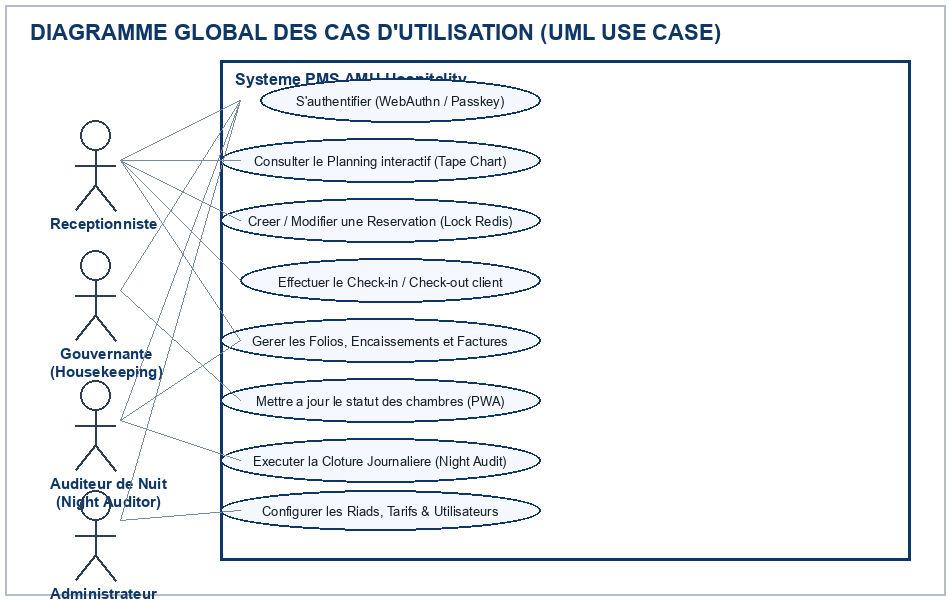
\includegraphics[width=0.95\textwidth]{figures/usecase_pms.png}
\caption{Diagramme global des cas d'utilisation du système PMS AMH Hospitality}
\label{fig:usecase_pms}
\end{figure}

Comme l'illustre la Figure~\ref{fig:usecase_pms}, les cas d'utilisation sont regroupés par domaine fonctionnel et reliés aux acteurs correspondants, avec des relations d'inclusion (\textit{<<include>>}) pour l'authentification obligatoire et la création de folio lors de la réservation.

\section{Description textuelle des cas d'utilisation majeurs}

\subsection{Cas d'utilisation CU01 : Créer une réservation}

Le Tableau~\ref{tab:uc_cu01} présente la fiche descriptive textuelle du cas d'utilisation CU01.

\begin{table}[H]
\centering
\small
\renewcommand{\arraystretch}{1.2}
\begin{tabularx}{\textwidth}{|p{3.5cm}|X|}
\hline
\textbf{Code \& Titre} & \textbf{CU01 -- Créer une réservation} \\
\hline
\textbf{Objectif} & Enregistrer un nouveau séjour client avec verrouillage distribué anti-collision sous Redis, initialisation du folio financier et diffusion temps réel de l'événement. \\
\hline
\textbf{Acteur(s)} & Réceptionniste (principal), Système PMS \\
\hline
\textbf{Précondition} & Réceptionniste authentifié. La chambre sélectionnée est libre sur l'intervalle de dates demandé au sein du Riad actif. \\
\hline
\textbf{Scénario nominal} & 
1. Le réceptionniste accède au planning Tape Chart et clique sur une plage de dates pour une chambre donnée.\\
& 2. Le système ouvre le modal de réservation et pré-remplit les dates et la catégorie de suite.\\
& 3. Le réceptionniste recherche et sélectionne un client existant (ou saisit une nouvelle fiche voyageur).\\
& 4. Le réceptionniste choisit le plan tarifaire applicable (ex: Standard avec petit-déjeuner inclus).\\
& 5. Dès validation du formulaire, le système tente d'acquérir un verrou distribué Redis sur la ressource \texttt{lock:room:\{id\}} avec un bail TTL de 10 secondes.\\
& 6. Le verrou étant accordé, le système ouvre une transaction SQL sous PostgreSQL, insère l'enregistrement dans la table \texttt{bookings} au statut \texttt{CONFIRMED} et génère un compte \texttt{folio} initial.\\
& 7. La transaction est validée (\textit{Commit}). Le système libère immédiatement le verrou Redis.\\
& 8. Le service publie un événement \texttt{booking.created} sur le bus RabbitMQ.\\
& 9. Le serveur diffuse une notification WebSocket à tous les clients connectés pour actualiser instantanément le Tape Chart.\\
& 10. Le système affiche un toast de confirmation de création avec l'identifiant du séjour.\\
\hline
\textbf{Scénarios alternatifs} & 
A1 -- \textit{Création d'un nouveau client} : À l'étape 3, si le voyageur n'existe pas dans le référentiel, le réceptionniste saisit son nom, prénom, nationalité et numéro de passeport, ce qui déclenche la création préalable de l'entité \texttt{Guest}.\\
& A2 -- \textit{Réservation multi-chambres (Groupe)} : Le réceptionniste associe plusieurs chambres au même dossier de réservation principal.\\
\hline
\textbf{Scénarios d'exception} & 
E1 -- \textit{Chambre en cours de réservation (Conflit de verrou)} : À l'étape 5, le verrou Redis ne peut être acquis car un autre opérateur tente de réserver la même chambre. Le système renvoie un code HTTP 409 Conflict et affiche un message d'alerte avec proposition de chambres équivalentes.\\
& E2 -- \textit{Erreur d'intégrité ou panne réseau} : En cas d'échec SQL à l'étape 6, la transaction subit un Rollback complet, le verrou Redis est nettoyé et un message d'erreur est affiché sans débit financier.\\
\hline
\end{tabularx}
\caption{Description textuelle du cas d'utilisation CU01 -- Créer une réservation}
\label{tab:uc_cu01}
\end{table}

\subsection{Cas d'utilisation CU02 : Effectuer le Check-in voyageur}

Le Tableau~\ref{tab:uc_cu02} présente la fiche descriptive textuelle du cas d'utilisation CU02.

\begin{table}[H]
\centering
\small
\renewcommand{\arraystretch}{1.2}
\begin{tabularx}{\textwidth}{|p{3.5cm}|X|}
\hline
\textbf{Code \& Titre} & \textbf{CU02 -- Effectuer le Check-in voyageur} \\
\hline
\textbf{Objectif} & Enregistrer l'arrivée physique du client, vérifier la conformité du statut ménage de la suite, contrôler les pièces d'identité réglementaires et activer le folio. \\
\hline
\textbf{Acteur(s)} & Réceptionniste (principal), Système PMS \\
\hline
\textbf{Précondition} & Réceptionniste authentifié. Réservation existante au statut \texttt{CONFIRMED}. La date d'arrivée correspond à la Business Date courante de l'établissement. \\
\hline
\textbf{Scénario nominal} & 
1. Le réceptionniste sélectionne la réservation du jour depuis la liste des arrivées attendues sur le tableau de bord.\\
& 2. Le système affiche le dossier complet : identité du voyageur, dates de séjour, chambre allouée et solde prévisionnel.\\
& 3. Le système interroge le service Housekeeping et vérifie que la chambre allouée est au statut \texttt{CLEAN} ou \texttt{INSPECTED}.\\
& 4. Le réceptionniste vérifie le passeport physique du client et saisit ou confirme le numéro de passeport / CIN et la date d'expiration pour la fiche de police.\\
& 5. Le réceptionniste clique sur le bouton « Valider le Check-in ».\\
& 6. Le système met à jour le statut de la réservation en \texttt{IN\_HOUSE} et horodate l'arrivée.\\
& 7. Le système active le compte \texttt{folio} pour permettre les imputations de consommations directes.\\
& 8. Le système publie un événement \texttt{guest.checked\_in} sur RabbitMQ et actualise le Tape Chart en temps réel.\\
& 9. Le système affiche un toast de confirmation et propose l'impression de la fiche d'enregistrement.\\
\hline
\textbf{Scénarios alternatifs} & 
A1 -- \textit{Changement de chambre à l'arrivée (Room Shift)} : Si la chambre initialement prévue présente une indisponibilité technique, le réceptionniste sélectionne une autre suite propre de catégorie identique ou surclassée (\textit{Upgrade}).\\
\hline
\textbf{Scénarios d'exception} & 
E1 -- \textit{Chambre non nettoyée (Statut DIRTY)} : À l'étape 3, si la chambre est encore marquée \texttt{DIRTY} ou \texttt{CLEANING\_IN\_PROGRESS}, le système bloque la validation du check-in et affiche une notification avec proposition d'alerter la gouvernante via la PWA.\\
& E2 -- \textit{Arrivée anticipée (Early Check-in)} : Si le client arrive avant l'heure standard, le système vérifie si la nuitée précédente était occupée et demande une confirmation avec éventuel supplément tarifaire.\\
\hline
\end{tabularx}
\caption{Description textuelle du cas d'utilisation CU02 -- Effectuer le Check-in voyageur}
\label{tab:uc_cu02}
\end{table}

\subsection{Cas d'utilisation CU03 : Exécuter la clôture journalière (Night Audit)}

Le Tableau~\ref{tab:uc_cu03} présente la fiche descriptive textuelle du cas d'utilisation CU03.

\begin{table}[H]
\centering
\small
\renewcommand{\arraystretch}{1.2}
\begin{tabularx}{\textwidth}{|p{3.5cm}|X|}
\hline
\textbf{Code \& Titre} & \textbf{CU03 -- Exécuter la clôture journalière (Night Audit)} \\
\hline
\textbf{Objectif} & Exécuter la clôture financière automatisée de la journée d'exploitation, facturer en masse les nuitées et taxes locales, figer les écritures comptables et incrémenter la Business Date. \\
\hline
\textbf{Acteur(s)} & Auditeur de Nuit (principal), Système PMS \\
\hline
\textbf{Précondition} & Auditeur authentifié avec rôle \texttt{NIGHT\_AUDITOR} ou \texttt{MANAGER}. L'ensemble des départs prévus ont été traités et les arrivées non honorées ont été qualifiées (No-Show ou report). \\
\hline
\textbf{Scénario nominal} & 
1. L'auditeur de nuit accède à l'interface « Clôture Journalière / Night Audit ».\\
& 2. Le système exécute une pré-vérification automatique et affiche la synthèse des contrôles : départs clôturés, arrivées traitées, folios en cours.\\
& 3. L'auditeur confirme les paramètres et clique sur « Lancer la Clôture Automatique ».\\
& 4. Le système initie une transaction globale distribuée :
   a. Pour chaque réservation active (\texttt{IN\_HOUSE}) sur la Business Date courante, le système calcule le tarif de la nuitée, la TVA (10\%), la Taxe de Séjour (25 MAD $\times$ nb adultes) et la Taxe de Promotion Touristique (12 MAD $\times$ nb adultes) ;
   b. Les écritures de débit correspondantes sont insérées dans la table \texttt{folio\_transactions} avec horodatage immuable et référence de la date d'exploitation ;
   c. Les soldes cumulés des folios sont recalculés et persistés.\\
& 5. Le système compile l'ensemble des données d'exploitation du jour et génère le rapport financier de clôture (\textit{Manager Daily Report}) au format PDF normalisé.\\
& 6. Le fichier PDF est archivé de manière immuable sur le stockage objet MinIO S3 sous la clé \texttt{reports/\{establishment\_id\}/audit\_\{date\}.pdf}.\\
& 7. Le système incrémente la date d'exploitation (\texttt{business\_date} $= \texttt{business\_date} + 1$).\\
& 8. La transaction globale est validée (\textit{Commit}).\\
& 9. Un événement \texttt{night\_audit.completed} est diffusé sur RabbitMQ et le bilan d'exécution est affiché à l'écran avec la durée totale de traitement (ex: 45 secondes).\\
\hline
\textbf{Scénarios d'exception} & 
E1 -- \textit{Blocage sur départ non effectué} : À l'étape 2, si un séjour dont le check-out était prévu aujourd'hui est toujours au statut \texttt{IN\_HOUSE}, le système bloque la clôture et exige une régularisation (prolongation ou départ).\\
& E2 -- \textit{Erreur d'intégrité transactionnelle} : En cas d'échec sur l'imputation d'un folio, la transaction entière subit un Rollback, la Business Date reste inchangée et un journal d'erreurs détaillé est affiché pour correction.\\
\hline
\end{tabularx}
\caption{Description textuelle du cas d'utilisation CU03 -- Exécuter la clôture journalière}
\label{tab:uc_cu03}
\end{table}

\subsection{Cas d'utilisation CU04 : Mettre à jour le statut ménage d'une chambre}

Le Tableau~\ref{tab:uc_cu04} présente la fiche descriptive textuelle du cas d'utilisation CU04.

\begin{table}[H]
\centering
\small
\renewcommand{\arraystretch}{1.2}
\begin{tabularx}{\textwidth}{|p{3.5cm}|X|}
\hline
\textbf{Code \& Titre} & \textbf{CU04 -- Mettre à jour le statut ménage (Housekeeping)} \\
\hline
\textbf{Objectif} & Permettre au personnel d'étage d'actualiser l'état d'entretien d'une chambre depuis un smartphone et propager instantanément le statut vers la réception. \\
\hline
\textbf{Acteur(s)} & Gouvernante / Femme de chambre (principal), Système PMS \\
\hline
\textbf{Précondition} & Gouvernante authentifiée sur l'application mobile PWA. La chambre existe dans l'établissement sélectionné. \\
\hline
\textbf{Scénario nominal} & 
1. La gouvernante ouvre la PWA Housekeeping sur son terminal mobile.\\
& 2. Le système affiche la liste des chambres assignées avec leur statut visuel courant (pastille de couleur).\\
& 3. La gouvernante sélectionne la chambre (ex: Suite Royale 101) et clique sur le nouveau statut (ex: \texttt{CLEAN} après nettoyage ou \texttt{INSPECTED} après vérification).\\
& 4. L'application mobile envoie une requête PATCH asynchrone vers l'endpoint \texttt{/api/v1/housekeeping/rooms/\{id\}/status}.\\
& 5. Le service Housekeeping valide la transition d'état selon la machine à états autorisée et met à jour la table \texttt{rooms}.\\
& 6. Le service publie un événement \texttt{room.status\_changed} sur le topic exchange RabbitMQ.\\
& 7. Le serveur WebSocket relaye l'événement à tous les navigateurs de réception connectés.\\
& 8. La pastille d'état de la chambre vire instantanément au vert sur le Tape Chart de réception sans rechargement de page.\\
& 9. La PWA confirme l'enregistrement par un retour haptique et visuel.\\
\hline
\textbf{Scénarios alternatifs} & 
A1 -- \textit{Signalement de maintenance} : La gouvernante bascule la chambre en \texttt{OUT\_OF\_ORDER} et saisit un commentaire décrivant l'avarie (ex: climatisation défaillante).\\
\hline
\textbf{Scénarios d'exception} & 
E1 -- \textit{Transition d'état invalide} : Tentative de passage direct de \texttt{DIRTY} à \texttt{INSPECTED} sans validation de nettoyage intermédiaire ; le système refuse et affiche un message de conformité.\\
\hline
\end{tabularx}
\caption{Description textuelle du cas d'utilisation CU04 -- Mettre à jour le statut ménage}
\label{tab:uc_cu04}
\end{table}

\section{Diagrammes de séquence dynamiques}

\subsection{Authentification biométrique sans mot de passe WebAuthn / Passkey}

La Figure~\ref{fig:seq_auth} détaille l'ordonnancement cryptographique des messages lors de l'authentification WebAuthn FIDO2 par appairage QR code.

\begin{figure}[H]
\centering
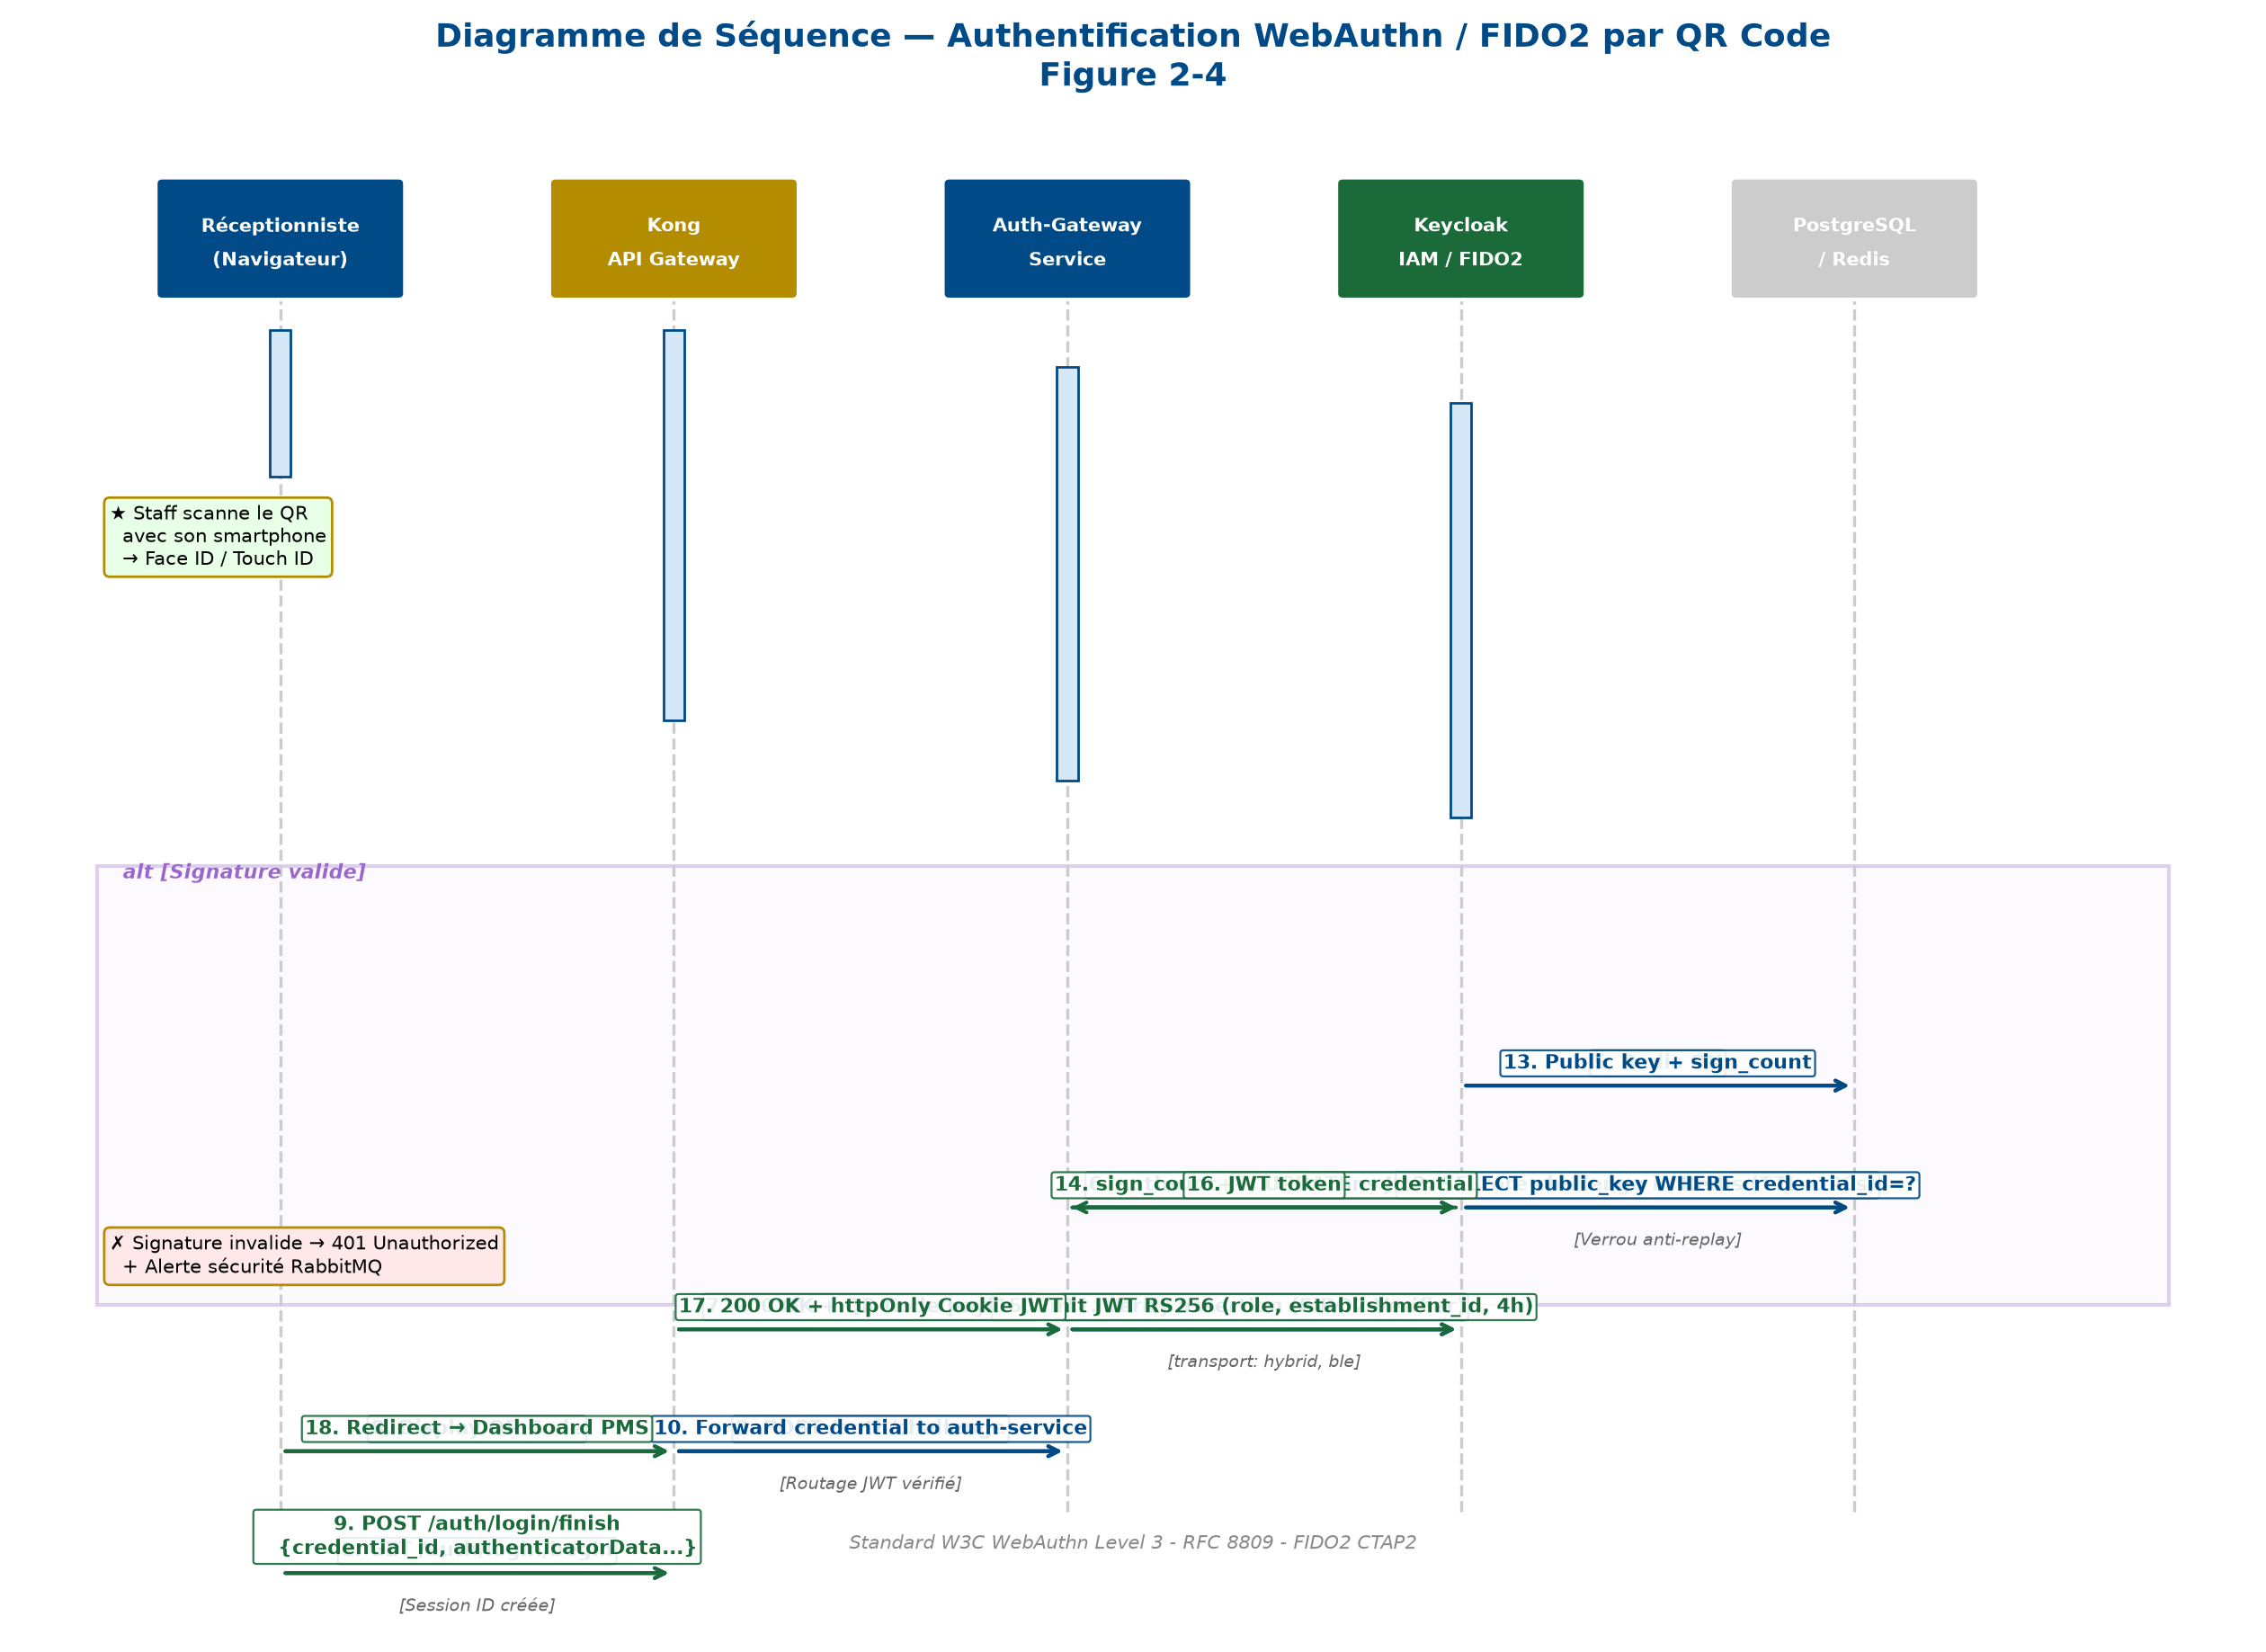
\includegraphics[width=0.95\textwidth]{figures/seq_auth.png}
\caption{Diagramme de séquence « Authentification WebAuthn / Passkey »}
\label{fig:seq_auth}
\end{figure}

Le flux illustré dans la Figure~\ref{fig:seq_auth} se déroule selon les étapes suivantes :
\begin{enumerate}
    \item Le réceptionniste clique sur « Connexion Passkey QR » sur le poste fixe de réception ;
    \item Le frontend Next.js sollicite l'API Gateway Kong qui achemine la requête vers le service \texttt{Auth Service} ;
    \item Le service interroge le serveur Keycloak FIDO2 qui génère un challenge cryptographique aléatoire de 32 octets et initialise une session d'appairage éphémère ;
    \item Le challenge et l'identifiant de session sont retournés au navigateur sous la forme d'un QR code dynamique affiché à l'écran ;
    \item Le réceptionniste scanne le QR code avec son smartphone personnel, ce qui ouvre le flux de signature WebAuthn sur le navigateur mobile sécurisé ;
    \item Le terminal mobile sollicite le capteur biométrique (TouchID ou FaceID) pour déverrouiller la clé privée stockée dans l'enclave sécurisée du smartphone (\textit{Secure Enclave}) et signe le challenge ;
    \item L'assertion signée est transmise à Keycloak qui valide la signature cryptographique à l'aide de la clé publique enregistrée ;
    \item L'assertion étant valide, Keycloak émet un jeton JWT d'accès signé asymétriquement (RS256) contenant l'identifiant de l'utilisateur, son rôle (\texttt{RECEPTIONIST}) et l'identifiant du Riad assigné ;
    \item Le poste de réception reçoit le jeton par canal sécurisé et redirige automatiquement l'utilisateur vers son tableau de bord d'exploitation.
\end{enumerate}

\subsection{Création de réservation et verrouillage distribué Redis}

La Figure~\ref{fig:seq_reservation} présente le diagramme de séquence de la création d'une réservation concurrente.

\begin{figure}[H]
\centering
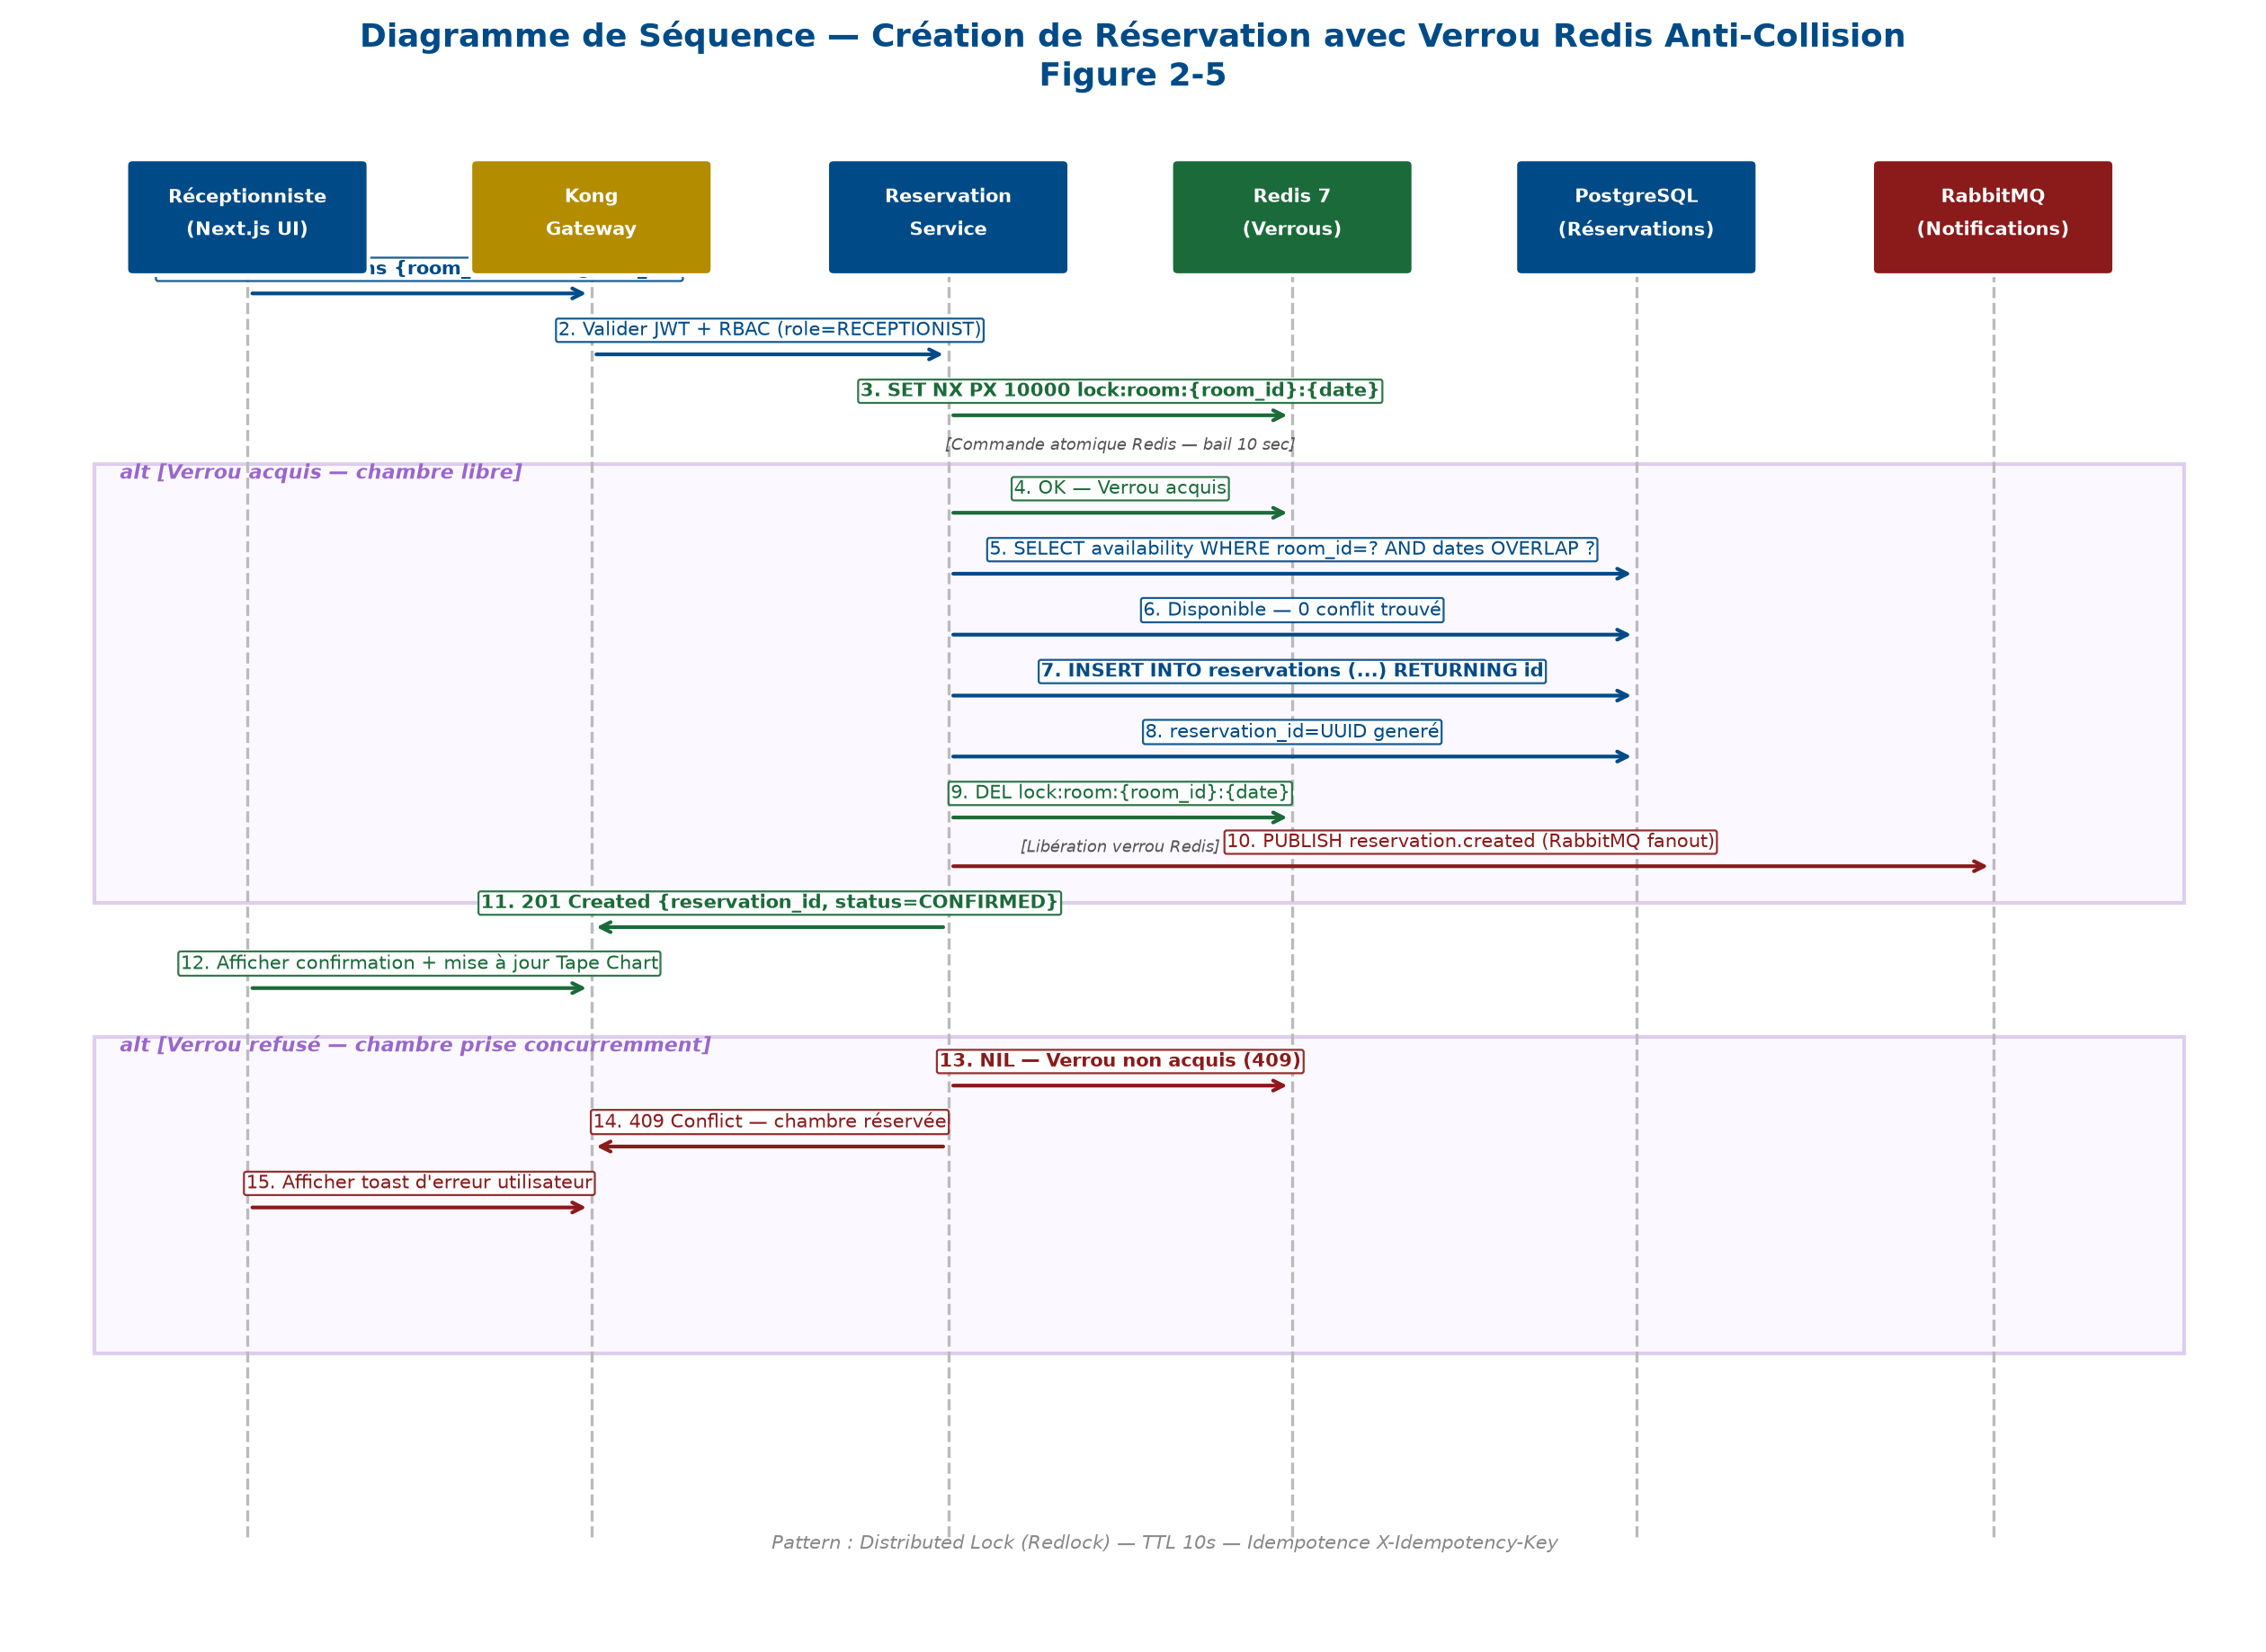
\includegraphics[width=0.95\textwidth]{figures/seq_reservation.png}
\caption{Diagramme de séquence « Création de réservation et Verrouillage Redis »}
\label{fig:seq_reservation}
\end{figure}

La Figure~\ref{fig:seq_reservation} met en lumière le rôle central du gestionnaire de verrous Redis :
\begin{enumerate}
    \item Le réceptionniste soumet le formulaire de réservation via une requête HTTP POST contenant les dates, l'identifiant de chambre, les informations client et une clé d'idempotence unique (\texttt{Idempotency-Key}) ;
    \item Le service \texttt{Reservation Service} tente d'acquérir un verrou distribué atomique sous Redis via la commande \texttt{SET lock:room:\{id\} \{uuid\} NX PX 10000} ;
    \item Si le verrou est obtenu avec succès, le service ouvre une transaction PostgreSQL, vérifie la non-collision dans la table \texttt{bookings}, effectue les insertions du séjour et du folio associé, puis valide la transaction (\textit{Commit}) ;
    \item Le verrou Redis est immédiatement libéré à l'aide d'un script Lua vérifiant la correspondance de l'identifiant UUID du propriétaire du verrou ;
    \item Le service renvoie un statut HTTP 201 Created et diffuse l'événement de réservation sur le topic RabbitMQ pour actualiser en temps réel le Tape Chart de tous les utilisateurs connectés.
\end{enumerate}

\subsection{Clôture journalière nocturne (Night Audit)}

La Figure~\ref{fig:seq_nightaudit} détaille le diagramme de séquence de la clôture automatisée Night Audit.

\begin{figure}[H]
\centering
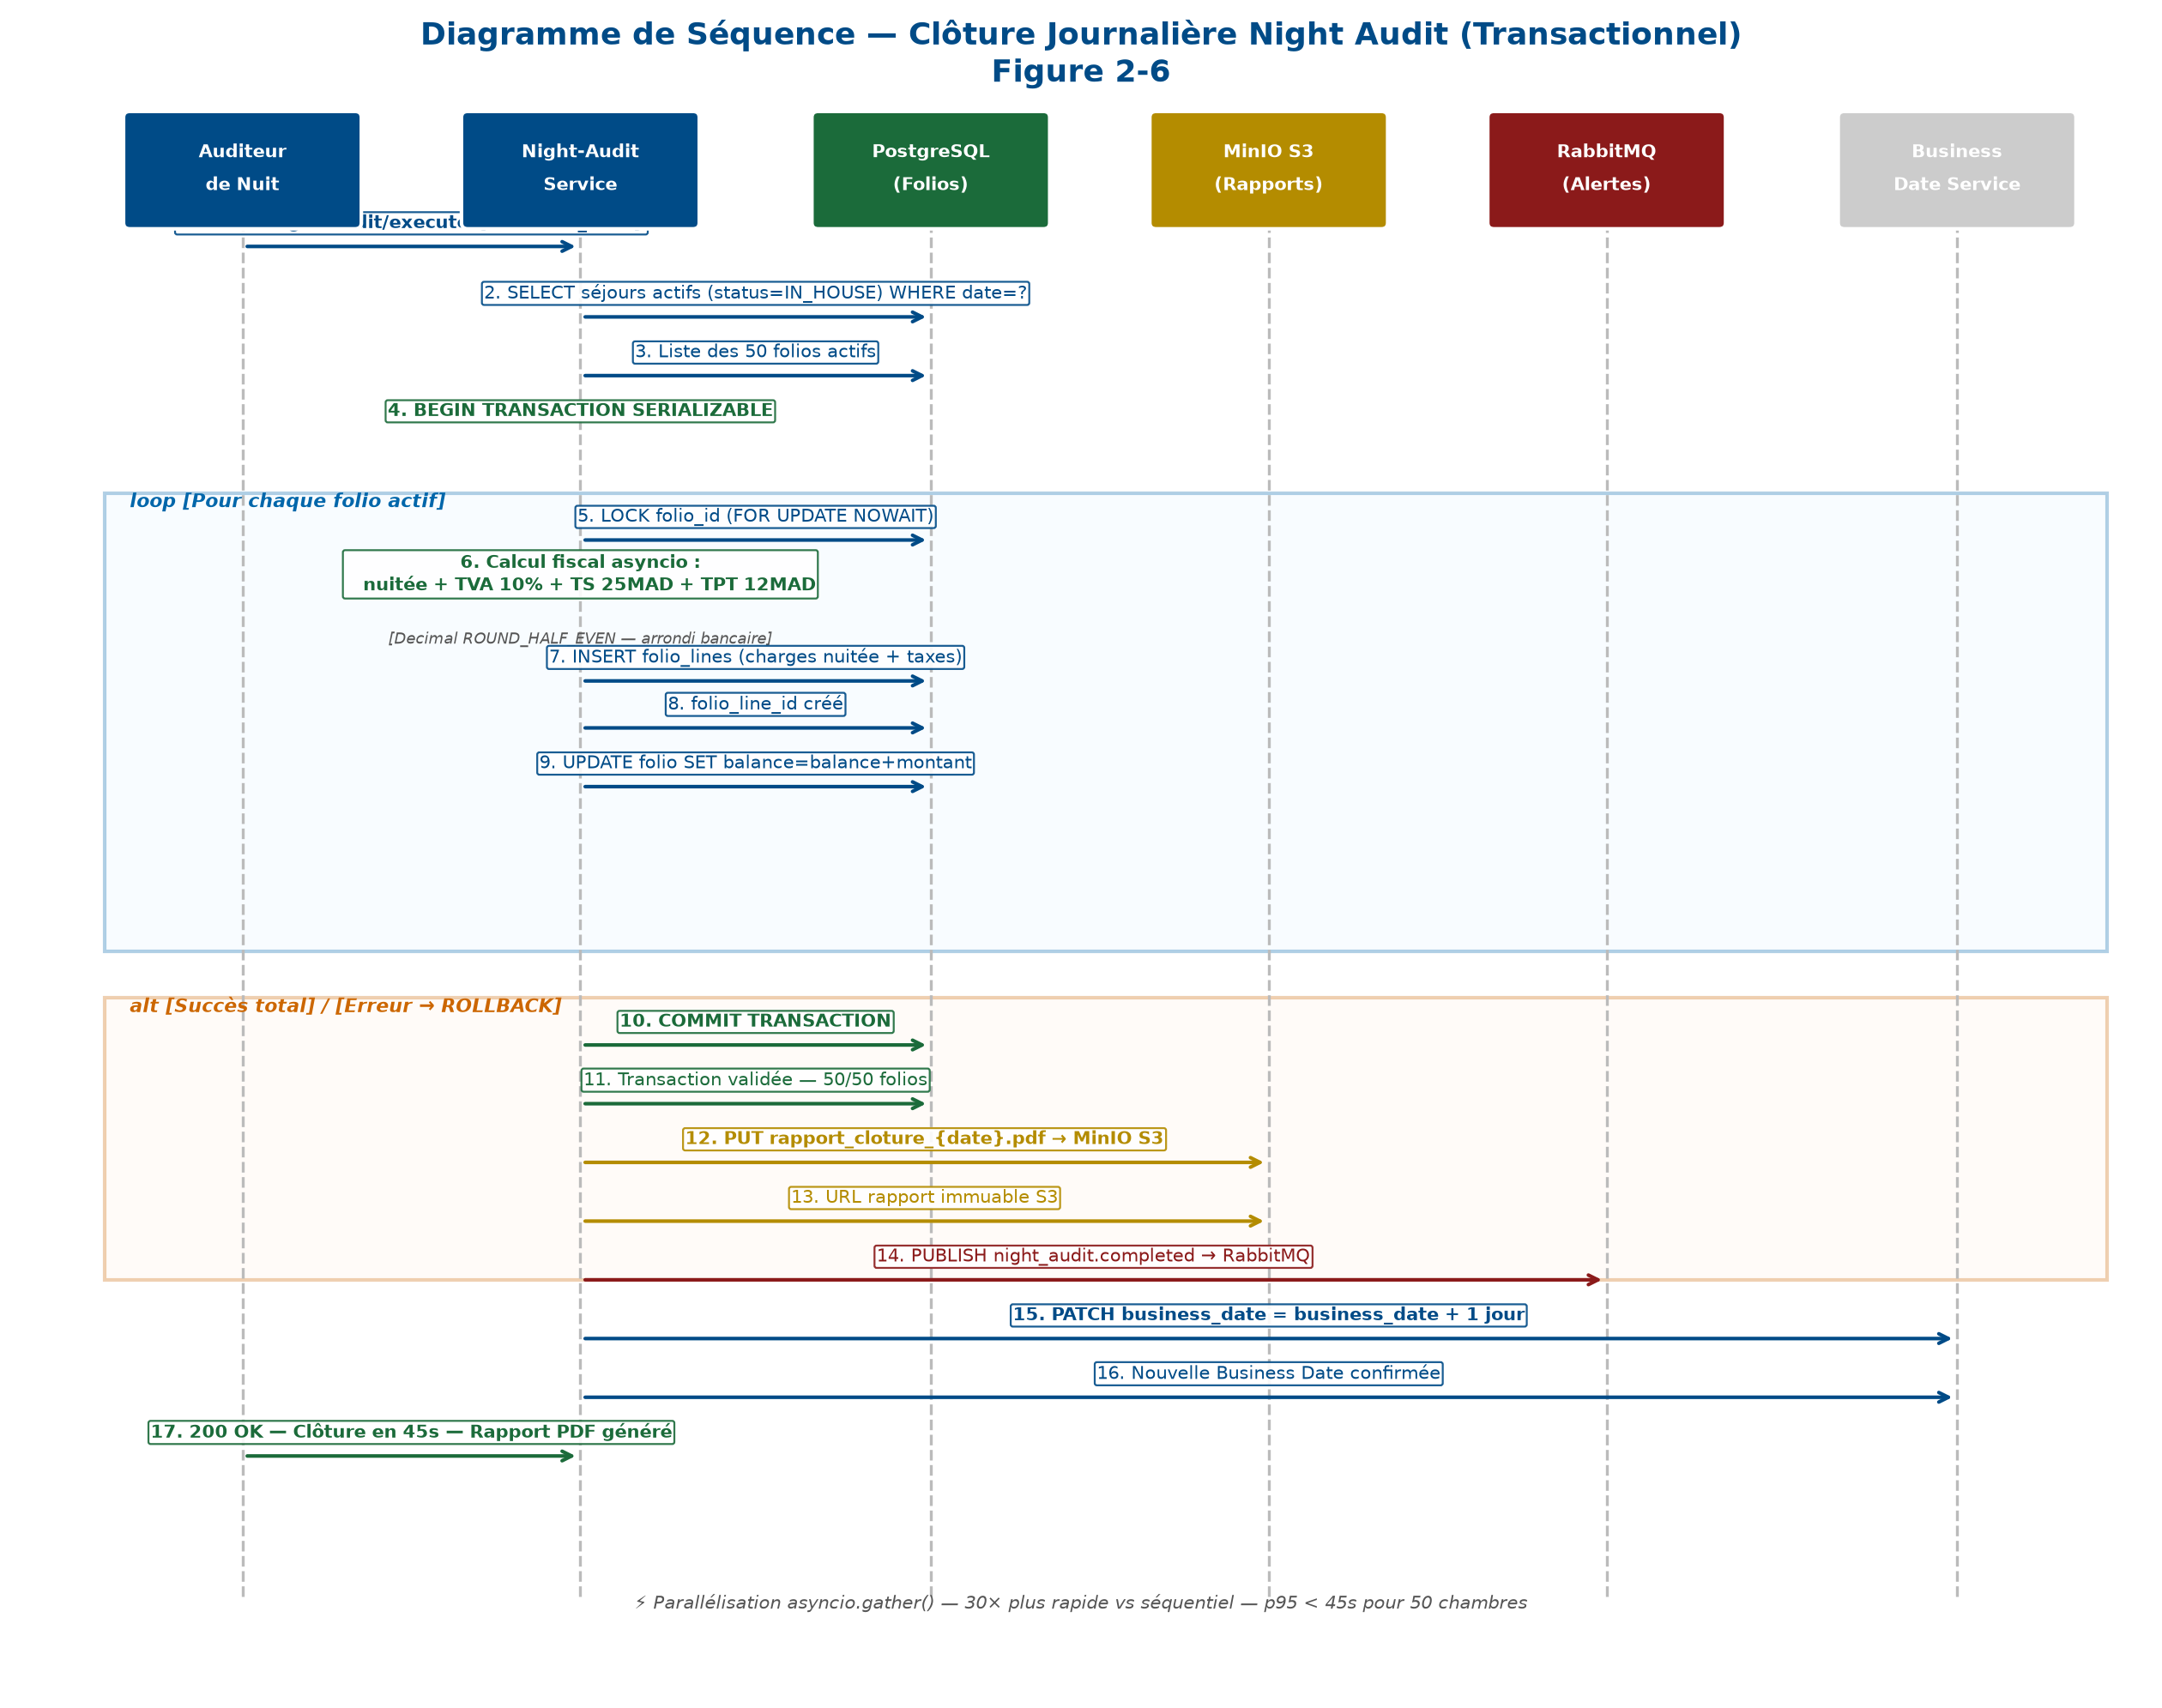
\includegraphics[width=0.95\textwidth]{figures/seq_nightaudit.png}
\caption{Diagramme de séquence « Clôture journalière Night Audit »}
\label{fig:seq_nightaudit}
\end{figure}

\section{Diagramme de classes du domaine métier hôtelier}

La Figure~\ref{fig:class_diagram_pms} expose le diagramme de classes UML représentant l'ontologie métier complète de la plateforme PMS AMH Hospitality.

\begin{figure}[H]
\centering
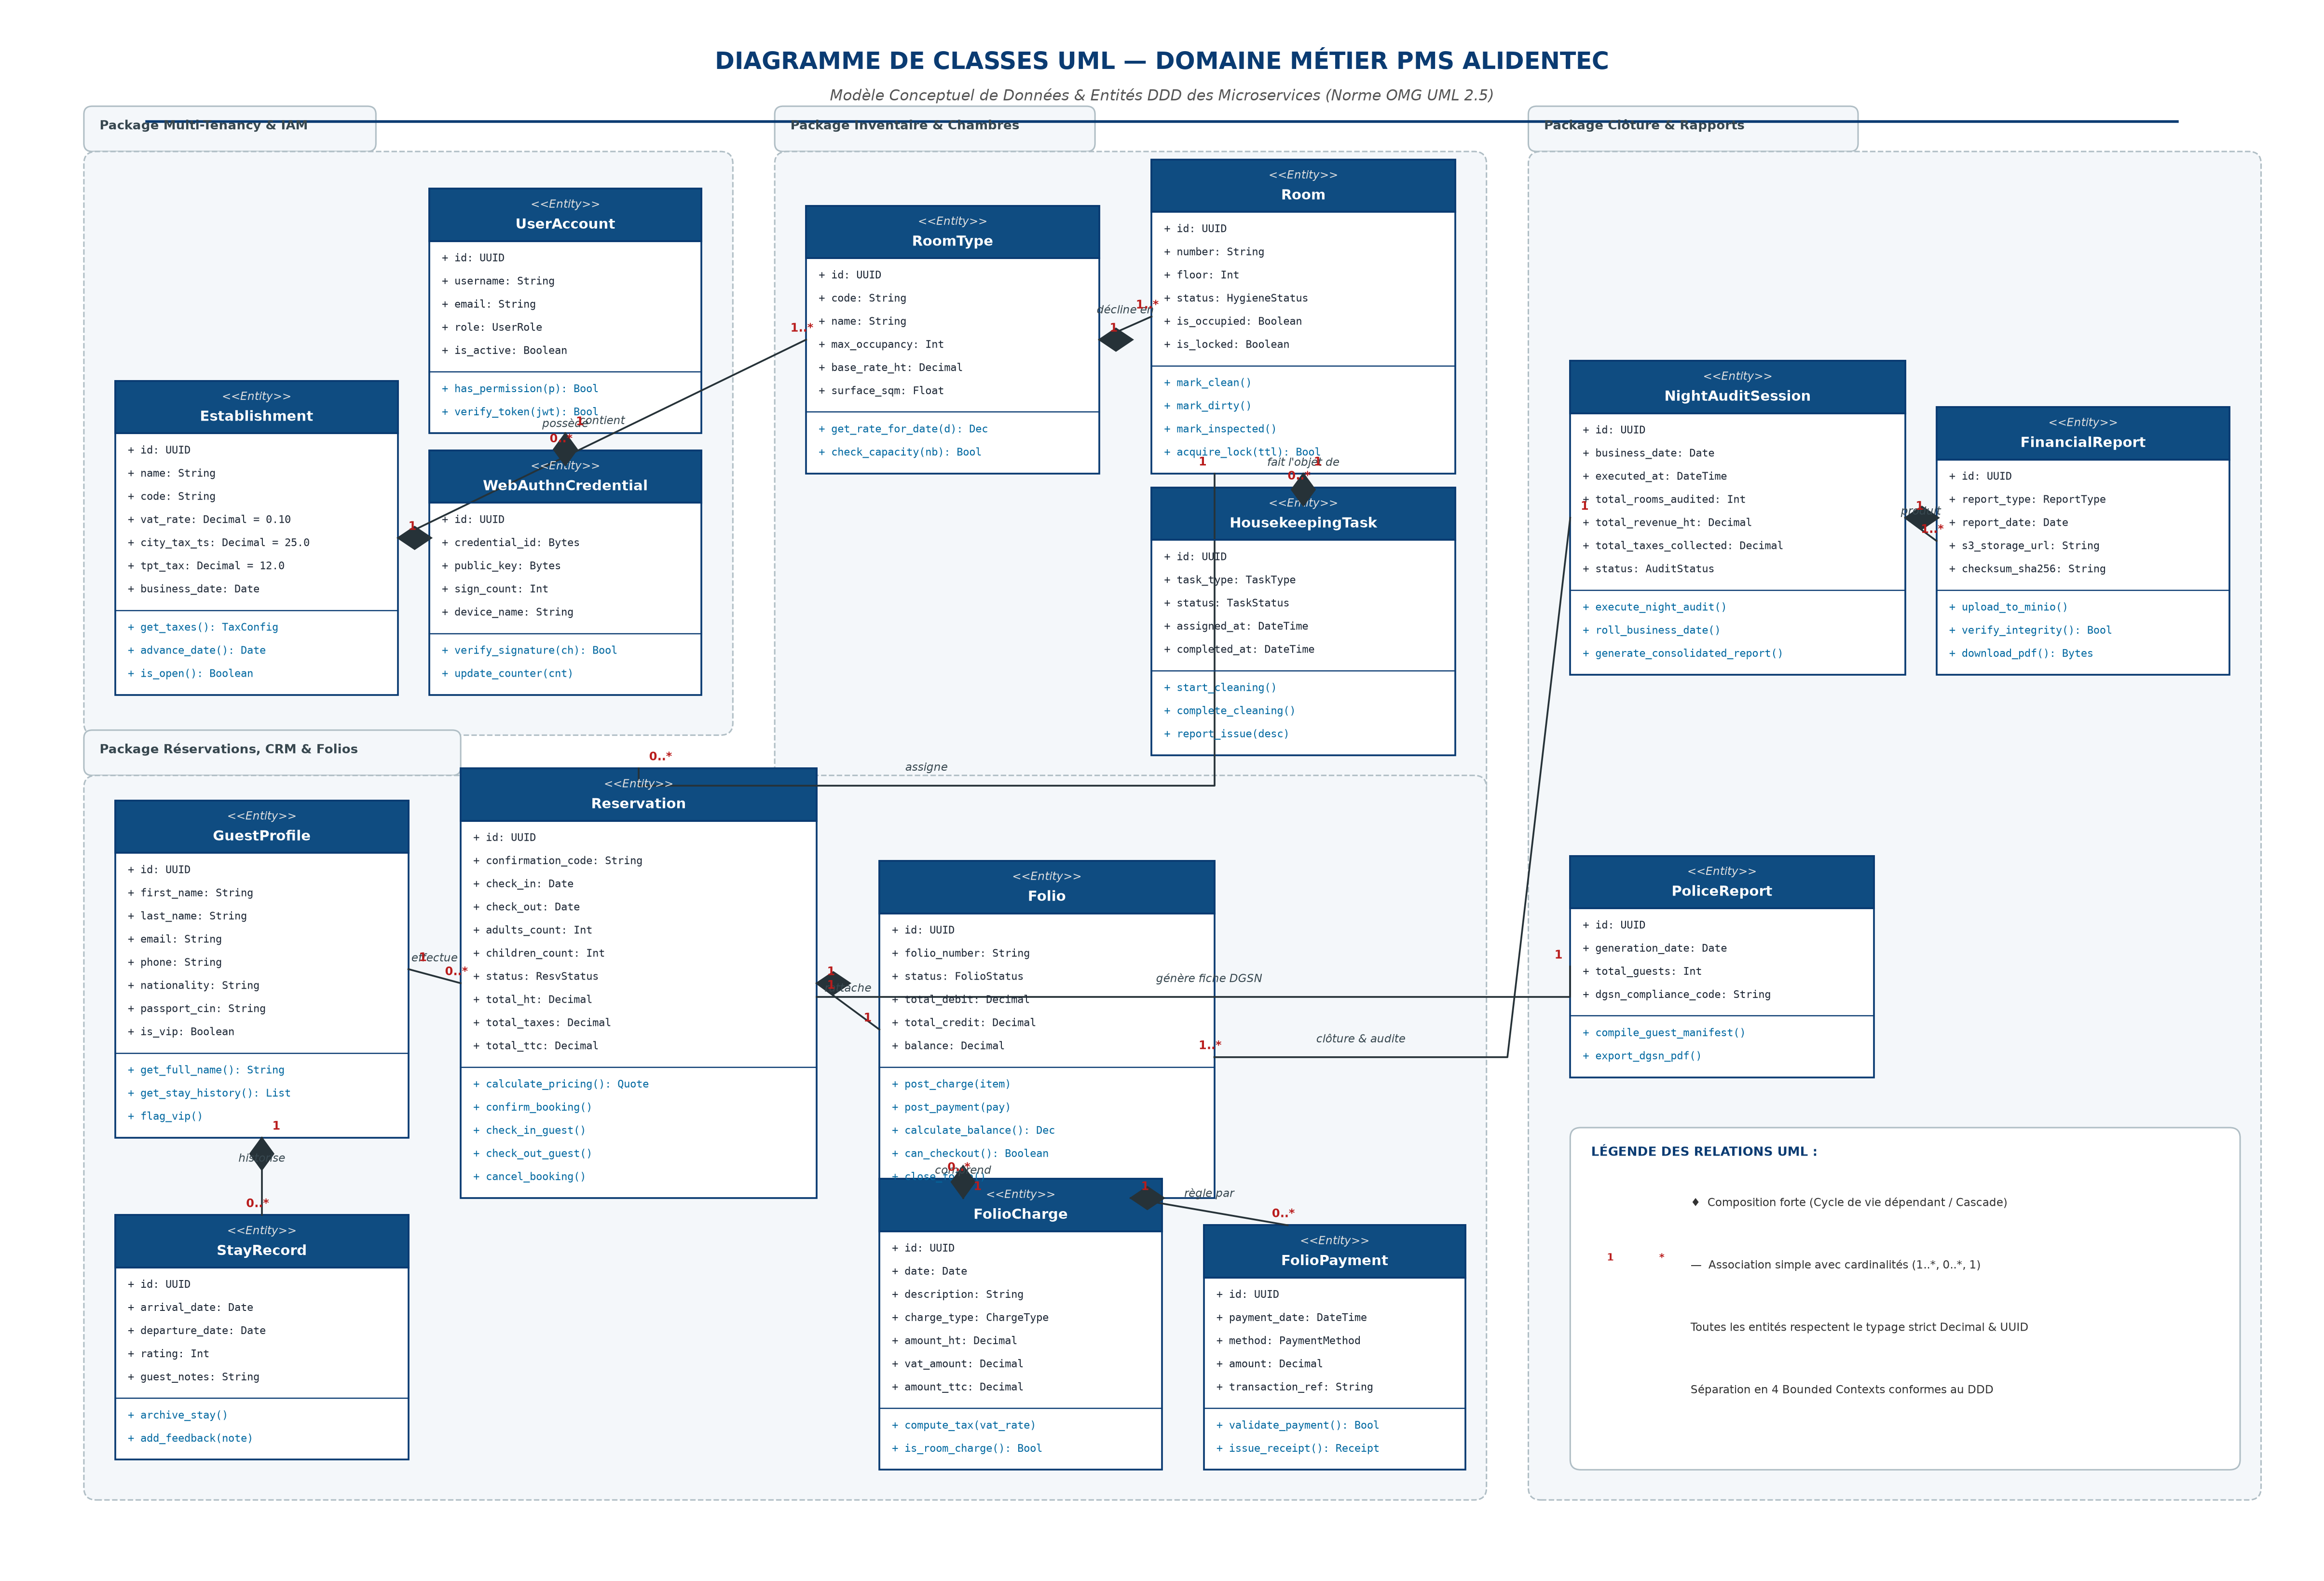
\includegraphics[width=0.95\textwidth]{figures/class_diagram_pms.png}
\caption{Diagramme de classes du domaine métier PMS AMH Hospitality}
\label{fig:class_diagram_pms}
\end{figure}

\subsection{Description détaillée des entités du domaine}

Le modèle de classes (Figure~\ref{fig:class_diagram_pms}) est structuré autour des entités métier fondamentales :

\begin{itemize}
    \item \textbf{Establishment (Établissement / Riad)} : Entité racine modélisant chaque propriété du groupe hôtelier.
    \begin{itemize}
        \item \textit{Attributs} : \texttt{id} (UUID), \texttt{name} (String), \texttt{code} (String unique, ex: \texttt{RYAS} pour Riad Yasmine), \texttt{city} (String), \texttt{address} (String), \texttt{business\_date} (Date), \texttt{vat\_rate} (Decimal = 0.10), \texttt{tourism\_tax} (Decimal = 25.00), \texttt{promotion\_tax} (Decimal = 12.00), \texttt{currency} (String = \texttt{MAD}) ;
        \item \textit{Méthodes} : \texttt{advanceBusinessDate() : Date}, \texttt{calculateTaxes(nights, guests) : TaxBreakdown}, \texttt{getActiveRooms() : List<Room>} ;
        \item \textit{Relations} : Composition forte 1 vers 1..* avec \texttt{Room} et 1 vers 0..* avec \texttt{RatePlan}.
    \end{itemize}
    
    \item \textbf{Room (Chambre / Suite)} : Représente chaque unité d'hébergement physique au sein d'un Riad.
    \begin{itemize}
        \item \textit{Attributs} : \texttt{id} (UUID), \texttt{establishment\_id} (UUID), \texttt{room\_number} (String), \texttt{category} (Enum : \texttt{SUITE\_ROYALE}, \texttt{SUITE\_JUNIOR}, \texttt{CHAMBRE\_DELUXE}, \texttt{CHAMBRE\_TRADITIONNELLE}), \texttt{floor} (Integer), \texttt{base\_capacity} (Integer), \texttt{max\_capacity} (Integer), \texttt{status} (Enum : \texttt{HousekeepingStatus}) ;
        \item \textit{Méthodes} : \texttt{updateHousekeepingStatus(new\_status)}, \texttt{isAvailableForDates(check\_in, check\_out) : Boolean}, \texttt{acquireLock(ttl) : Boolean} ;
        \item \textit{Relations} : Appartient à un \texttt{Establishment}, associée à 0..* \texttt{Booking}.
    \end{itemize}

    \item \textbf{RatePlan (Plan Tarifaire)} : Définit la grille tarifaire applicable selon les conditions de vente.
    \begin{itemize}
        \item \textit{Attributs} : \texttt{id} (UUID), \texttt{establishment\_id} (UUID), \texttt{name} (String), \texttt{code} (String), \texttt{base_price} (Decimal), \texttt{is\_refundable} (Boolean), \texttt{includes\_breakfast} (Boolean), \texttt{min\_stay} (Integer) ;
        \item \textit{Méthodes} : \texttt{calculateDailyRate(date, occupancy) : Decimal}.
    \end{itemize}

    \item \textbf{Guest (Voyageur / Client)} : Consigne les informations d'identité et l'historique du voyageur.
    \begin{itemize}
        \item \textit{Attributs} : \texttt{id} (UUID), \texttt{first\_name} (String), \texttt{last\_name} (String), \texttt{email} (String), \texttt{phone} (String), \texttt{nationality} (String), \texttt{id\_document\_type} (Enum : \texttt{PASSPORT}, \texttt{CIN}), \texttt{id\_document\_number} (String), \texttt{vip\_tier} (Integer : 0=Standard, 1=Silver, 2=Gold, 3=VIP Royal) ;
        \item \textit{Méthodes} : \texttt{getFullName() : String}, \texttt{getBookingHistory() : List<Booking>}.
    \end{itemize}

    \item \textbf{Booking (Réservation / Séjour)} : Centralise les paramètres contractuels et opérationnels du séjour.
    \begin{itemize}
        \item \textit{Attributs} : \texttt{id} (UUID), \texttt{establishment\_id} (UUID), \texttt{guest\_id} (UUID), \texttt{room\_id} (UUID), \texttt{rate\_plan\_id} (UUID), \texttt{check\_in\_date} (Date), \texttt{check\_out\_date} (Date), \texttt{adults\_count} (Integer), \texttt{children\_count} (Integer), \texttt{status} (Enum : \texttt{CONFIRMED}, \texttt{IN\_HOUSE}, \texttt{CHECKED\_OUT}, \texttt{CANCELLED}, \texttt{NO\_SHOW}), \texttt{total\_amount} (Decimal), \texttt{channel} (String : \texttt{DIRECT}, \texttt{BOOKING\_COM}, \texttt{AIRBNB}), \texttt{idempotency\_key} (String) ;
        \item \textit{Méthodes} : \texttt{confirm()}, \texttt{checkIn()}, \texttt{checkOut()}, \texttt{roomShift(new\_room, reason)}, \texttt{cancel(reason)}.
    \end{itemize}

    \item \textbf{Folio (Compte Facture)} : Gère la balance comptable et financière du séjour.
    \begin{itemize}
        \item \textit{Attributs} : \texttt{id} (UUID), \texttt{booking\_id} (UUID), \texttt{status} (Enum : \texttt{OPEN}, \texttt{CLOSED}, \texttt{BALANCED}), \texttt{total\_debit} (Decimal), \texttt{total\_credit} (Decimal), \texttt{balance} (Decimal), \texttt{opened\_at} (DateTime), \texttt{closed\_at} (DateTime) ;
        \item \textit{Méthodes} : \texttt{postCharge(amount, category, desc, vat)}, \texttt{postNightlyRate(rate, ts, tpt)}, \texttt{registerPayment(amount, method)}, \texttt{isBalanced() : Boolean} ;
        \item \textit{Relations} : Composition forte 1 vers 0..* avec \texttt{FolioTransaction}.
    \end{itemize}

    \item \textbf{FolioTransaction (Ligne d'Écriture Financière)} : Enregistre chaque mouvement financier individuel.
    \begin{itemize}
        \item \textit{Attributs} : \texttt{id} (UUID), \texttt{folio\_id} (UUID), \texttt{timestamp} (DateTime), \texttt{amount} (Decimal), \texttt{vat\_amount} (Decimal), \texttt{category} (Enum : \texttt{ROOM\_NIGHT}, \texttt{TOURISM\_TAX}, \texttt{RESTAURANT}, \texttt{SPA\_WELLNESS}, \texttt{LAUNDRY}, \texttt{PAYMENT}), \texttt{description} (String), \texttt{transaction\_type} (Enum : \texttt{DEBIT}, \texttt{CREDIT}), \texttt{user\_id} (UUID -- traçabilité de l'opérateur).
    \end{itemize}
\end{itemize}

\section{Cartographie des contextes délimités (Domain-Driven Design)}

Conformément aux principes architecturaux du \textit{Domain-Driven Design} (DDD) d'Eric Evans, le domaine complexe de la gestion hôtelière multi-riads a été décomposé en contextes délimités (\textit{Bounded Contexts}) autonomes, garantissant une séparation stricte des responsabilités et une étanchéité des modèles de données :

\begin{enumerate}
    \item \textbf{Identity \& Access Context (Auth Service)} : Gestion des utilisateurs, des clés d'accès WebAuthn, des sessions et des permissions RBAC ;
    \item \textbf{Establishment Structure Context (Establishment Service)} : Référentiel des Riads, des suites, des équipements, de la Business Date et des taux fiscaux ;
    \item \textbf{Guest Relationship Context (Guest Profile Service)} : Répertoire unifié des voyageurs, fidélité VIP et préférences personnalisées ;
    \item \textbf{Booking \& Inventory Context (Reservation Service)} : Moteur d'inventaire des chambres, gestion des disponibilités, tarification et verrous Redis anti-overbooking ;
    \item \textbf{Front-Office Operations Context (Front-Office Service)} : Processus d'accueil, Check-in, Check-out, fiches de police et réattributions de chambres (Room Shift) ;
    \item \textbf{Billing \& Folio Accounting Context (Billing Service)} : Comptes folios, imputation des charges et extras, calculs fiscaux (TVA, TS, TPT) et factures PDF ;
    \item \textbf{Night Audit Automation Context (Night Audit Service)} : Moteur de clôture nocturne transactionnel, agrégation financière et archivage S3 ;
    \item \textbf{Housekeeping Operations Context (Housekeeping Service)} : Gestion de la propreté d'étage, statuts de chambres et notifications WebSockets ;
    \item \textbf{Event Notification Context (Notification Service)} : Diffusion des alertes et événements en temps réel via le bus RabbitMQ ;
    \item \textbf{Distribution \& Channel Management Context (Channel Manager)} : Passerelle de synchronisation bidirectionnelle avec les OTA externes ;
    \item \textbf{Reporting \& Strategic Analytics Context (Reporting Service)} : Calcul des indicateurs de performance hôtelière consolidés (RevPAR, ADR, taux d'occupation).
\end{enumerate}

\section{Conclusion}

Ce deuxième chapitre a permis d'établir une modélisation formelle, exhaustive et structurée de la plateforme logicielle \textbf{PMS AMH Hospitality}. À travers l'étude critique de l'existant, la matrice RACI des acteurs, le diagramme des cas d'utilisation, les fiches descriptives textuelles détaillées, les diagrammes de séquence dynamiques et le diagramme de classes du domaine métier articulé en contextes délimités DDD, l'ensemble des règles métier a été rigoureusement spécifié. Le chapitre suivant sera consacré à la description détaillée de l'environnement technique, des frameworks, des bases de données et des protocoles de communication API REST mis en œuvre pour donner corps à cette conception.
